%----------------------------------------------------------------------------------------
%	PACKAGES AND OTHER DOCUMENT CONFIGURATIONS
%----------------------------------------------------------------------------------------

\documentclass[twoside]{article}

\usepackage{lipsum} % Package to generate dummy text throughout this template

\usepackage[sc]{mathpazo} % Use the Palatino font
\usepackage[T1]{fontenc} % Use 8-bit encoding that has 256 glyphs
\usepackage[utf8]{inputenc}
\linespread{1.05} % Line spacing - Palatino needs more space between lines
\usepackage{microtype} % Slightly tweak font spacing for aesthetics
\usepackage{graphicx}

\usepackage[hmarginratio=1:1,top=32mm,columnsep=20pt]{geometry} % Document margins
\usepackage{multicol} % Used for the two-column layout of the document
\usepackage[hang, small,labelfont=bf,up,textfont=it,up]{caption} % Custom captions under/above floats in tables or figures
\usepackage{booktabs} % Horizontal rules in tables
\usepackage{float} % Required for tables and figures in the multi-column environment - they need to be placed in specific locations with the [H] (e.g. \begin{table}[H])
\usepackage{hyperref} % For hyperlinks in the PDF

\usepackage{lettrine} % The lettrine is the first enlarged letter at the beginning of the text
\usepackage{paralist} % Used for the compactitem environment which makes bullet points with less space between them

\usepackage{abstract} % Allows abstract customization
\renewcommand{\abstractnamefont}{\normalfont\bfseries} % Set the "Abstract" text to bold
\renewcommand{\abstracttextfont}{\normalfont\small\itshape} % Set the abstract itself to small italic text

\usepackage{titlesec} % Allows customization of titles
\renewcommand\thesection{\Roman{section}} % Roman numerals for the sections
\renewcommand\thesubsection{\Roman{subsection}} % Roman numerals for subsections
\titleformat{\section}[block]{\large\scshape\centering}{\thesection.}{1em}{} % Change the look of the section titles
\titleformat{\subsection}[block]{\large}{\thesubsection.}{1em}{} % Change the look of the section titles

\usepackage{amsmath}
\usepackage{algpseudocode}
\usepackage{algorithm}

\newcommand{\todo}[1]{\textbf{TODO(#1)}}
\renewcommand{\v}[1]{\vec{#1}}

%----------------------------------------------------------------------------------------
%	TITLE SECTION
%----------------------------------------------------------------------------------------

% otsikosta saa 2/40 p
% A search for well-performing algorithms  
\title{\vspace{-15mm}\fontsize{24pt}{10pt}\selectfont\textbf{Prediction of wine type and quality using chemical characteristics}}

\author{
\large
\textsc{A search for well-performing algorithms in type and quality prediction}\\[2mm]
\textsc{Hannu Siikonen, Mikko Perttunen}\\[2mm]
\vspace{-5mm}
}
\date{}

%----------------------------------------------------------------------------------------

\begin{document}

\maketitle % Insert title

%----------------------------------------------------------------------------------------
%	ABSTRACT
%----------------------------------------------------------------------------------------

\begin{abstract}
% myöskin 2/40 p, 100-200 sanaa
The type and quality of wines is to be predicted using machine learning techniques. The prediction
of type is a pure classification problem, but the prediction of quality can be viewed both as
a classification or a regression problem. Various classification algorithms are equipped
for the analyses of the two problems and also some regression algorithms are used for the study
of the quality. It turns out that the prediction of the type is a problem that can be solved
with an excellent accuracy. A hybrid model is constructed for making the final predictions
of the type. On the contrary, determining the quality of a wine is challenging. Different
algorithms are tested out and the final result is obtained using only one learning
algorithm. The obtained model performs somewhat well, but there is room for optimization. 
The results are satisfactory, but this kind of a machine learning problem provides a source
for endless study.

\end{abstract}

%----------------------------------------------------------------------------------------
%	ARTICLE CONTENTS
%----------------------------------------------------------------------------------------

\begin{multicols}{2} % Two-column layout throughout the main article text

\section{Introduction}
% 4/40 p
% Introduces the reader to the topic and the broad context within which the research fits
% Why is the task important, what question is being addressed, what is hoped to learn?
% Literature review

The goal of this study is to predict the type and the quality of a wine by making use of a given dataset.
This is realized by comparing the strengths and weaknesses of different machine learning 
and statistical modeling algorithms when applied to the present data. Optimized learning algorithms
are then revised based on the performance of the different methods.
 
All possible algorithms cannot be considered in these analyses. Nevertheless,
a variety of methods is used. This is important when dealing with a randomly chosen dataset, since according to
Wolpert \todo{\LaTeX-viittaus}, there is no simple way to predetermine which
learning algorithm yields the best results with the data. It can be difficult to assess,
which method has an inductive bias that corresponds best to the data.
The evaluated algorithms were selected based on their diversity and using some initial hypotheses.

For the sake of variety, the performance of both regression and classification algorithms is evaluated.
However, the focus is on classification algorithms. 
Both the prediction of the type and the quality of the wine can be considered
classification problems, whereas only the quality can be studied also using regression. It is obvious that
there is some correlation between neighboring classes, that is, quality values that differ by only one point. This implies that
using regression is a good idea. On the other hand the integer presentation of the quality makes using regression cumbersome.

The used dataset is derived from the so called \emph{Vinho verde} dataset by Cortez et al. \cite{CorCer09}.
It consists of 6000 observations, each describing an individual wine. For each one of them, 11 variables are provided in addition
to the color and the quality of the wine: fixed acidity, volatile acidity, density, pH and amounts of citric acid, residual sugar, chlorides, 
free sulfur dioxide, total sulfur dioxide, sulphates and alcohol in the wine. The type of each wine is either red or white 
and the quality is an integer between 1 and 7. 5000 observations are used as training data, while the other 1000 are reserved for testing.

Wine data is in general a favored object for study in the field of machine learning. There have been various studies
on the subject, for instance those by Cortez et al. \cite{WQA}, \cite{CorCer09} 
and Appalsamy et al. \cite{Appalsami}. One motive for this are the large and growing markets of the wine industry.
Being able to predict the quality of a wine without the need for a wine taster, as well as a deeper understanding
of the properties of a good wine, induce much potential for profit. On the other hand, the problem of predicting
the quality of a wine is intriguing from a machine learning perspective. The quality is determined by human taste,
a very complex and subjective system, difficult to predict only by using a limited set of chemical properties.
One more reason to explain the popularity of wine quality predictions is the fact that there is a lot of data
on wines available on the Internet.

This task is interesting, since the prediction problem is twofold: both a clear physical property and an abstract, subjective property
are to be predicted. The former should be relatively easily predictable, assuming that a sufficient set
of chemical properties is given. The prediction of the quality, on the other hand, can be a very challenging task.
In general, these kinds of hard problems are often ones that are good for benchmarking machine learning algorithms.
In addition to that, with such difficult problems a great interest exists for a decently performant prediction algorithm,
since prior to sufficient computing power and analysis methods they have been insolvable. Thus, this study provides a
good review of the features of modern machine learning algorithms when applied to a complex dataset.
 
\section{Methods}
% 8/40 p
% Methods used to conduct your experiment
% Concept-level: Methods/algos and modifications to these

For predicting the behavior of the wine data multiple machine learning methods are equipped.
To some extent the same classification algorithms with minor differences are used for both
the analysis of the type and the analysis of the quality of wines. On top of this, to augur the 
quality, some regression algorithms are utilized. The basic properties of the used algorithms
are described in this section. The theoretical background of most of the algorithms can be found
in a basic reference, such as Ref. \cite{Alpaydin}. 

\subsection{Classification}

\subsubsection{Naive Gaussian discrimination} \label{method:naiivig}

While taking initial steps with a dataset, it is usually instructive to begin with a simple
learning algorithm. This could mean using a model that always returns a constant value or
class. A slightly more complicated simple model is provided by using only one of the eleven prediction variables
given in the data. The initial hypothesis is that for some of the variables ($x$) all classes are somewhat
normally distributed. It follows that by calculating the mean value 
$\mu$ and variance $\sigma^2$ of each class using the training set, the probability distributions of 
each class $k$ is obtained:
\begin{equation}
 p(x|\mu_k,\sigma_k) = \frac{1}{\sqrt{2\pi} \sigma_k} e^{-\frac{(x-\mu_k)^2}{2\sigma_k^2}}.
\end{equation}
This can be used directly as a likelihood function for the different classes. Also a Bayesian posterior
can be taken:
\begin{equation}\label{posterior}
 p(\mu_k,\sigma_k|x) \propto p(x|\mu_k,\sigma_k) p(\mu_k,\sigma_k),
\end{equation}
where $p(\mu_k,\sigma_k) = p(\theta_k)$ is simply obtained as the fraction of the class $k$ in the 
training set. This can be transformed conveniently into a discriminant, by choosing a reference
class $j = k$:
\begin{equation}\label{naiividiskr}
 g_k(x) = \log \frac{p(\mu_k,\sigma_k|x)}{p(\mu_j,\sigma_j|x)}.
\end{equation}
The maximal $g_k(x)$ indicates the predicted class $k$. By simplifying Eq. \eqref{naiividiskr},
it is obtained
\begin{equation}\label{naiividiskr2}
 g_k(x) = \frac{(x-\mu_j)^2}{2\sigma_k^2}-\frac{(x-\mu_k)^2}{2\sigma_k^2} + 
 \log \frac{\sigma_j}{\sigma_k}.
\end{equation}

\subsubsection{Multivariate Gaussian discrimination}\label{method:multig}

The multivariate Gaussian discriminant operates analogically to the one-dimensional
case, extending the discriminant function to eleven variables. It determines the class of a sample by
comparing the probabilities of it belonging to each class, when each
class is modeled using a multivariate Gaussian distribution. This can be problematic,
since many real-world variables have a clearly non-Gaussian distribution.

The Gaussian distributions are determined based on training data.
The mean vector $\v{\mu}_k$ and covariance matrix $\mathbf{\Sigma}_k$ are calculated for each class.
The probability of a sample $x$ belonging to the class can then be calculated
using the multivariate Gaussian probability density function:

\begin{equation}\label{monigauss}
 p(\v{x}|\v{\mu}_k,\mathbf{\Sigma_k}) = \frac{1}{\sqrt{2\pi} |\mathbf{\Sigma_k}|}
 e^{-\frac{1}{2}(\v{x}-\v{\mu}_k)^T \mathbf{\Sigma}_k^{-1} (\v{x}-\v{\mu}_k)}
\end{equation}

The likelihood of Eq. \eqref{monigauss} can be used directly for estimating the class of a
sample $\v{x}$, or a Bayesian posterior can be utilized as in Eq. \eqref{posterior}. 
A discriminant can be constructed parallelly to Eqs. \eqref{naiividiskr} and \eqref{naiividiskr2}:
\begin{equation}
	\begin{aligned}
	 g_k(\v{x}) = \frac{1}{2}(\v{x}-\v{\mu}_j)^T \mathbf{\Sigma}_j^{-1} (\v{x}-\v{\mu}_j) - \\
	 \frac{1}{2}(\v{x}-\v{\mu}_k)^T \mathbf{\Sigma}_k^{-1} (\v{x}-\v{\mu}_k) 
	+\log \frac{|\mathbf{\Sigma}_j|}{|\mathbf{\Sigma}_k|}.
       \end{aligned}
\end{equation}
Again, the class with the largest discriminant $g_k(\v{x})$ indicates the prediction of class, $k$.

\subsubsection{$k$ nearest neighbours}\label{method:knn}

The $k$ nearest neighbours classifier is a non-parametric classifier. Only a
distance function between the points in the variable space is required.
The classification given by $k$ nearest neighbours for a new point $\v{x}$ is then found by 
selecting the $k$ points closest to $x$ according to the distance function and
picking the most common class among the $k$ points. The training set is fully
stored in memory. The samples in it are used for the nearest neighbour study
of the points in the validation or the test set.

Selecting a good distance function is important, especially when many variables
are used for the prediction. The distributions of the
input variables can vary greatly. When using the Euclidean distance function,
this causes certain variables to have a greater effect on the distance between
points when compared to others. To prevent this, we used the Mahalanobis
distance function\cite[p.~88]{Alpaydin}:

\begin{equation}\label{eq:mahalanobis}
  D_M(\v{x}, \v{y}) = \sqrt{(\v{x}-\v{y})^T \Sigma^{-1} (\v{x}-\v{y})},
\end{equation}

where $\Sigma$ is the covariance matrix $\v{x}$ int the training set.
This normalizes the distances in the different dimensions of
the variable space and also takes into account unnecessary correlations.
The Mahalanobis distance is an intuitive distance measure for an arbitrarily
scaled space. It appears for instance in the exponent of the multivariate
Gaussian distribution of Eq. \eqref{monigauss}.

If the class probabilities $p_c(\v{x})$ for a point $\v{x}$ are required, these can
be calculated using the nearest neighbours of it. If the frequency of a class $c$
within the $k$ nearest neighbours is $k_c$, the probability is simply
\begin{equation}
 p(\v{x}) = \frac{k_c}{k}.
\end{equation}

\subsubsection{Linear discrimination}\label{method:ldiskr}

Methods that rely on discrimination can model directly the class discriminants instead of
the class probabilities. In linear discrimination the discriminant for a class $k$ is linear:
\begin{equation}
 g_k(\v{x}) = \v{w}_k^T v{x} + w_{k0}.
\end{equation}
The basic theory of linear discrimination is not deeper than this: the goal is to find such
coefficients $\v{w}_k$, $w_{k0}$ that the classification error is minimal. Usually this has
to be done numerically for instance with the steepest descent algorithm. There are multiple 
ways to perform the optimization. One example
is logistic discrimination, in which the class probabilities are defined by a connection to the class
probabilities. The discriminant of a class $k$ is a logarithm of the fraction of the likelihood of
this class divided by the likelihood of a reference class. This definition gives some convenient 
properties for the model from the viewpoint of numerical solutions. However, also other
approaches may be used.

\subsubsection{Quadratic discrimination}\label{method:qdiskr}

Quadratic discrimination is otherwise similar to linear discrimination, but it equips a quadratic discriminant function,
\begin{equation}
 g_k(\v{x}) = \v{x}^T \mathbf{W}_k \v{x} + \v{w}_k^T \v{x} + w_{k0}.
\end{equation}
Because of the quadratic form, the search for optimal discriminants is much more complicated than with linear
discriminants. Additionally, the additional complexity brought by the quadratic form may be unnecessary.
Nevertheless, quadratic discrimination provides a good algorithm for comparison, if an efficient algorithm
for it is available.

\subsubsection{Support vector machine}\label{method:svm}

Support vector machines are a variant of linear discrimination. If classes do not overlap, it finds
the separating hyperplanes between the classes that have the largest margins. These hyperplanes correspond 
to linear discriminants. With overlapping classes, a penalty term is added to the solution in order
to make the same approach work.

\subsubsection{Random forest}\label{method:randfor}

Random forest \cite{Forest} is an ensemble learning method that equips an ensemble of classification trees. Each tree 
in the ensemble does classification using only a chosen number of input variables. This could be for
instance the square root of the total amount of classification variables. For this kind of an ensemble of trees
the trees themselves are usually unpruned. The trees themselves are simply ordinary classification trees:
they use the given variables and split the branches until a desired amount of purity or other conditions
are fulfilled for the training set. It is important that there is a sufficient amount of classification
trees in the ensemble. With a too small amount of trees sufficient statistics is not reached and the algorithm
does not perform optimally.

\subsection{Regression}

\subsubsection{Random forest, regression}

The random forest algorithm can be used also for regression. In this case, the classification trees in the 
ensemble are substituted with regression trees. A regression tree has leaves with constant values,
since a typical tree cannot easily give continuous output. When an ensemble of regression trees is considered, the 
situation is more complicated. The final output is averaged over many trees and thus the output resembles
more a continuous behaviour.

\subsubsection{Linear least squares}\label{method:leastsquare}

The linear (or ordinary) least squares method is a regression algorithm that
finds a linear fit for one variable as a function of multiple variables: $\hat{y} = \v{a}^T \v{x}+b$. 
The vector $\v{a}$ and the constant $b$ are such that in the training set $\sum (y - \hat{y})$ is 
minimized, hence the name least squares.

The problem can be conveniently presented in a matrix form. Let $\mathbf{X}$ be a matrix
with rows $[1, \v{x}^T]$, composed of all the samples in the training set. That is, the 
constant $b$ is now included in the vector for the sake of convenience. Let $\v{y}$ be
a corresponding column vector and $\v{w}$ a column vector that holds the linear coefficients and
\begin{equation}
\hat{\v{y}} = \mathbf{X} \v{w}
\end{equation}
is the least squares estimate. The least squares problem is equal to minimizing the
vector product $(\v{y} - \hat{\v{y}})^T(\v{y} - \hat{\v{y}})$ with respect to $\v{w}$. 

It can be shown that the optimal solution is given by 
\begin{equation}
 \v{w} = (\mathbf{X}^T \mathbf{X})^{-1} \mathbf{X}^T y.
\end{equation}
In this form an arbitrary matrix $\mathbf{X}$ can be used. That is,
$\mathbf{X}$ may hold only the given variables in a basic form, but also for instance higher
exponents of the variables can be inserted into this matrix. Thus, it is relatively simple
to control the complexity of the model.

\subsection{PCA}\label{method:pca}

Primary Component Analysis is a method that can be used with both classification and regression
problems. Effectively, it reduces the amount of variables that the predicted variable depends
on. This can be useful, if some of the provided data is not at all useful in the analysis. On the other
hand, it gives an effective method of graphical representation of the data. If the studied variable
depends on over three dimensions, using PCA it can be projected to three or two dimensions.

PCA itself relies on finding new variables that are responsible for most of the variance of the studied
variable. The greater the effect on the variance, the more the parameter explains the behaviour of the variable.
Mathematically, PCA studies the covariance matrix of the matrix that holds the training set samples of the 
variables that are used to predict the variable of interest. The eigenvectors of the covariance matrix are
the principal components. The corresponding eigenvalues indicate the relative fraction of variance that
the principal components (eigenvectors) are responsible for. 

If PCA is done with a reduction from $N$ to
$K$ dimensions, the $K$ largest eigenvalues of the covariance matrix are chosen. The data in the training set is shifted so that
its mean value is zero in all dimensions, and then it is projected on the $K$ eigenvectors that correspond
to the chosen eigenvalues. This is the PCA-representation.

\subsection{Combining learners}\label{method:combo}

If many different learners with approximately equal performance are found, it is instructive
to combine these to boost the performance. For this, many kinds of algorithms can be used
but in this work a simple approach is taken. It is assumed that maximally three very good
learning algorithms are chosen for the final model. With these algorithms, the probabilities
of each class are calculated for each sample in the validation or testing set. The probabilities
are denoted with $P_1$, $P_2$ and $P_3$ and they are given weights $w_1$, $w_2$ and $w_3$.
The weights are normalized so that $w_1 + w_2 + w_3 = 1$. Thus the final probability is given by
\begin{equation}
 P = w_1 ( P_1 - P_3 ) + w_2 ( P_2 - P_3 ) + P_3.
\end{equation}
Because of the normalization condition and the assumption that the weights are greater than zero,  $0 \leq w_1,w_2 \leq$ and $w_1 + w_2 \leq 1$. 
An approximate solution can be found by scanning the possible values of $w_1$ and $w_2$ on a lattice with a spacing of $0.01$.
The best weights are chosen by validation. With only two learning algorithms, one parameter has to be scanned over.

%\begin{figure}[H]
%\centering
%\includegraphics[width=0.5\textwidth]{learning}
%\caption{Learning is important but big processors are importanter. \cite{alpaydin2004introduction}}
%\label{fig:learning}
%\end{figure}

%------------------------------------------------

\section{Experiments}
% 8/40 p
% Method and materials (applied)
% Necessary for applying the methods to the data: pre-proc., validation of params (cross-validation)
% No results here!

The study is divided into two different problems: the prediction of the type (color) and the quality (ranking)
of wines. Of these the latter is a considerably more demanding task, since the quality consists of more classes than the type and the
ruling mechanisms of the human taste are complicated. To probe the data, at first simple algorithms are used for 
both the tasks. This is a good way of keeping the analysis reasonable as
the hypothetically inferior algorithms give a starting level for the required performance. If a hypothetically
well-performing algorithm performs similarly as a naive algorithm, it can be rejected.

For the actual analysis, matlab is used for the most part. It would be possible to implement these algorithms by hand,
but it makes more sense to use the algorithms that are already supplied by matlab. This way, it is possible to focus
on the actual properties of the algorithms instead of programming them.

\subsection{Method validation}

Method validation is done using $k$-fold cross validation with $k = 10$. The training set is partitioned in 10 equally sized parts. 
Validation is done ten times using each partition once as a validation set, while the other nine
sections function as training sets. The mean error of the 10 different validations is used as a measure
of goodness of an algorithm.

Cross-validation can be a bit problematic if it is used both for choosing parameter values for a single algorithm (e.g., the value of $k$
for the kNN-algorithm) and evaluating the goodness of the different algorithm. In such a case the choice of the parameter value makes the estimator
of goodness biased, which is harmful when making decisions between the algorithms. However, with the given amount of data
the 10-fold cross-validation is a good choice. Since $9/10$ of the whole training data is used as a training set at a time,
the situation resembles that of the actual final training phase. While training the final algorithm, the whole training dataset
is used. On the other hand, the small size of a single validation set is averaged out by considering all 10 different validation sets.
The overlap of the ten training sets lowers the quality of validation slightly. Nonetheless, it is not easy to use a given amount
of training data more economically than with $k$-fold cross-validation.

\subsection{Algorithm evaluation}

While using learning algorithms, type is not used as a predictor for quality and quality not for color.
In principle, such a measure could be useful. If either quality or color was predicted very
accurately, there would be new information in the second decision process.
However, there is a great amount of uncertainty involved in using an already predicted value as a
variable of the second learner. If a test set differs significantly from the training set, this could
make the second algorithm perform poorly.

Some of the algorithms are used for the study of both problems while others are only applied to one of them.
Knowledge of chemistry or any other kind of preliminary knowledge of wines is not used. The tasks are treated purely as machine learning
problems. The greatest external utility in this context is the set of the variables that are used for the predictions,
which were supplied in beforehand. PCA and similar methods are useful
for studying, whether there is some useless variables in the given dataset. Additionally, the quality of the final testing results imply, whether the supplied
data was sufficient.

For evaluating the performance of different algorithms a couple of different methods are used. The 
most basic measure is the total amount of false augurs, when the problem is treated as classification.
This does not give a complete picture of the situation. For instance
with classification problems one can predict that all the samples in the test data belong to one class. If
this class has a high prior probability, it can be supposed that a large amount of predictions are correct.
However, this is problematic, since only the members of one class are predicted correctly. A simple algorithm
could give a similar error rate as the given naive assumption, but it would probably also have a non-zero success
rate for the other classes. This is preferable and hence a more complicated measure of goodness, \emph{f-score}, is used:
\begin{equation}
 \text{f-score} = \frac{ 2 \times \text{precision} \times \text{recall} }{\text{precision} + \text{recall}}.
\end{equation}
This measure is used for each class within the study. To get the total f-score of a prediction, a weighted sum of
the f-scores of the classes is taken. The weights are normalized and proportional to the amount of samples in
each class in the set that is being predicted. Here the following definitions are used:
\begin{eqnarray}
 &\text{precision} & = \frac{N_{tp}}{N_{tp}+N_{fp}} \\
 &\text{recall} & = \frac{N_{tp}}{N_{tp}+N_{fn}}.
\end{eqnarray}
The $N$ -quantities refer simply to the amounts of samples of certain types. The letter $t$ stands for true and $f$ for false.
Additionally $p$ stands for positive and $n$ for negative. By using this kind of a definition the evaluation of goodness
is more complicated than with a simple fraction of errors. The more correct predictions one class receives, the less it raises
the total f-score of an algorithm. On the other hand, a class with only a few correct predictions benefits much more from
a raise in the amount of true positives. Thus, using f-score, more value is given for the \emph{variety of classes}.

Since the prediction of quality has some regressive nature, an additional score more fitting for regression was given
for the forecasts of quality. The score is defined as the square root of the mean square error:
\begin{equation}\label{distmetric}
 \epsilon = \sqrt{\frac{1}{N} \sum_{i=1}^N ( \text{prediction}_i - \text{true}_i )^2 }.
\end{equation}
This score indicates how much the predicted quality differs from the actual quality. It is more of a curiosity than the other scores,
but it helps in obtaining a full picture of the situation.

\subsection{Prediction of type}

In principle the prediction of type is a task that is easily regressed to the chemical properties of a wine.
The most significant distinction between white and red wines is the color, which strongly implies that the type 
has its foundation in the fine structure of the wine.

\subsubsection{Simple classification methods}

The initial model that is used for the type is one that predicts a constant type for the wines. 
Since there are only two types available, this will by definition give an error rate that is below $50\%$. However,
at least the f-score should be relatively low.

As a first proper algorithm we use the naive Gaussian estimate as described in section \ref{method:naiivig}. With this it is
important to find a variable for which the types are somewhat distributed in the shape of a bell curve. The obtained 
result is a numerically non-challenging and simple prediction. From this the analysis can be logically extended to a full
multivariate Gaussian prediction, as shown in section \ref{method:multig}. This should work better than a univariate
Gaussian method even if the variables were not in general distributed in a Gaussian way. For both the multivariate
and univariate Gaussian cases also Bayesian prior probabilities are applied.

Thus, three initial methods are developed. None of these are actually expected to perform very well, since the inductive
biases are significant. However, now a solid basis is set for a further analyses.

\subsubsection{More involved classification methods}

There is actually no good initial knowledge on what kind of a classifier
would perform well in the given situation. Therefore, the algorithms have to be tested out. Here, some preliminary 
pruning has been performed in order to obtain a diverse set of algorithms.

The linear discriminant method is used to make a somewhat generic prediction for the classification. This divides the variable space
with hyperplanes, which separate each class to a confined area. While the algorithms of matlab are used, also a quadratic discriminant
could be in principle equipped. In general, this is not that advisable because the full quadratic form adds much unnecessary complexity
to the model.

To contribute to the results of a linear discriminant, also a $k$ Nearest Neighbours -model is used. In this case it is important to choose
a fitting value for the parameter $k$. The 10-fold cross-validation method is fitting for this choise. It should be noted that if the model
tends to be optimal with small values of $k$, its probability-related features are diminished. As an extreme, with $k=1$ the class probabilities
of a point in the test set are 0 or 100 $\%$. Probability-related properties are important while models are combined and thus also this aspect
should be taken into account.

As a last choice the Random Forest algorithm is used. It combines both ensemble methods and classification trees. For this algorithm both the size
of the forest and the amount of parameters used for classification has to be chosen. The size of the forest means the amount of trees in the ensemble.
Making this parameter larger is good for the results but it will increase the calculation time. For the amount of variables used in a single tree a
value clearly smaller than 11 should be used. This means approximately 4 or less variables. In general, less variables can be good so that
all variables are taken properly into account. On the other hand, less variables in a tree means a demand for using a larger forest. Thus,
with this algorithm matters related to computational time become important.

\subsubsection{PCA}

Primary component analysis can be useful in pre-processing data, at least if some \emph{unnecessary} data is given. Thus, it is good to check, whether
using it is beneficial with the current data. It can also depend on the algorithm, whether or not PCA gives enhanced results. The kNN-algorithm and random
forest in general are friendly with a high dimensionality. Thus, a reduction in dimensionality may not be very helpful. On the contrary, the linear discriminant
method may obtain significant advantage of having to use less dimensions. Thus, this method is tested with different amounts of projection dimensions.

\subsubsection{Combining algorithms}

If the performance of multiple algorithms is in the same scale, these algorithms should be combined to obtain even better results. It depends on the amount
of methods to be combined, how complex this process is. However, maximally 3 methods are combined and this can be done in the way described in section \ref{method:combo}.

\subsection{Prediction of Quality}

There are various possible problems that can arise in the prediction of the quality. One major issue is that it is
not known, whether it is more favorable to use classification or regression algorithms. This has to be tested
to some extent. In the classification there are some similarities to the 
prediction of the type with the distinction that many aspects are now more complicated.

\subsubsection{Classification}

A \emph{constant class} classifier is once again used but this time Gaussian classifiers are left out. 
Univariate classification is too simple to work well with seven classes.
On the other hand a full multivariate classification is cumbersome to use and is not worth the 
additional effort, since other algorithms are likely to work better.

Various dicriminative methods are used: linear discrimination, as well as the support vector machine and quadratic discrimination. 
It is instructive to probe different discrimination methods to determine whether they are useful in the current problem. 
The quadratic discriminant could be helpful in this case because of the complexity of the problem.

Additionally, also the $k$ Nearest Neighbors and random forest classification are used once again. In principle, there are only minor
differences when compared to the use of these algorithms in the case of type prediction.

\subsubsection{Regression}

While using regresion algorithms there are two relevant questions: how does a regression algorithm perform in the context
of regression and how does it perform in the context of classification. For the former, the additional score type was
given. If a regression algorithm seems to perform generally well, it may be used for the final model.

The random forest algorithm is powerful and it can be applied also for regression. Its usage is simple,
since the only difference to classification is that the final result is not an integer. The result is rounded to the nearest
integer, to make it compatible with the true qualities.

In addition, the least squares method is utilized, as shown in \ref{method:leastsquare}. This is somewhat compulsory, taking
into account that the least squares method is very popular in regression applications.

\subsubsection{PCA and Combining algorithms}

Based on the type prediction PCA results, it is determined whether it is useful to use PCA 
in this context. On the other hand, algorithm combination has the same rules as in the case of 
type. If there are algorithms that have a somewhat similar performance level, they should be
combined. If one algorithm is clearly better than the others, it can be used alone for the final predictions.

% \begin{table}[H]
% \caption{My current knowledge of tables}
% \centering
% \begin{tabular}{cc}
% \textbf{Table type} & \textbf{Likely location}\\
% \midrule
% Coffee table & Living room\\
% Dining table & Dining room\\
% Bedside table & Bedroom
% \end{tabular}
% \end{table}

%------------------------------------------------

\section{Results}
% 4/80 p
% Description of results with figures and tables

The analyses of algorithmical performance were carried out so that the type was analyzed before the quality. The final learning algorithms
were chosen by optimization among the used algorithms. Thus, there was \emph{communication} between obtaining results and enhancing the models.

\subsection{Prediction of type}

The performance of multiple algorithms was tested using cross validation on the training dataset and for comparison also the performance in the testing data was studied.
F-score and total error rate were calculated for the naive Gaussian discriminant, multivariate Gaussian discriminant, linear discrimination, $k$ Nearest Neighbors and random forest
algorithms, as well as for the final hybrid algorithm.
Since a majority of the test observations consists of white wines, an intuitive dummy model predicts that all wines are white. The performance of this dummy model
is also included in the results.

The training and testing datasets can be visualized by projecting into a two-dimensional plane using principal component analysis. The two most important
PCA components of the data are given in figures~\ref{fig:color_training_pca} (training set) and~\ref{fig:color_testing_pca} (test set). 
Blue dots are used for marking the white wines and red dots for marking the red wines.
For each evaluated algorithm, the rate of successful predictions and the f-score are reported. In addition, the success of the predictions is shown on PCA projections
of the observations. These are given in appendix \ref{appendix:colorpcakuvet}.

A sample of the code used for these tasks is given in appendix \ref{appendix:colorcode}. The code is from a cross-validation scheme for the different
algorithms. This gives a good view on the structure of the code used. Also other cross-validations were done similarly. The difference to the testing code is
that in testing there is no cross-validation loop.

\begin{figure}[H]
\centering
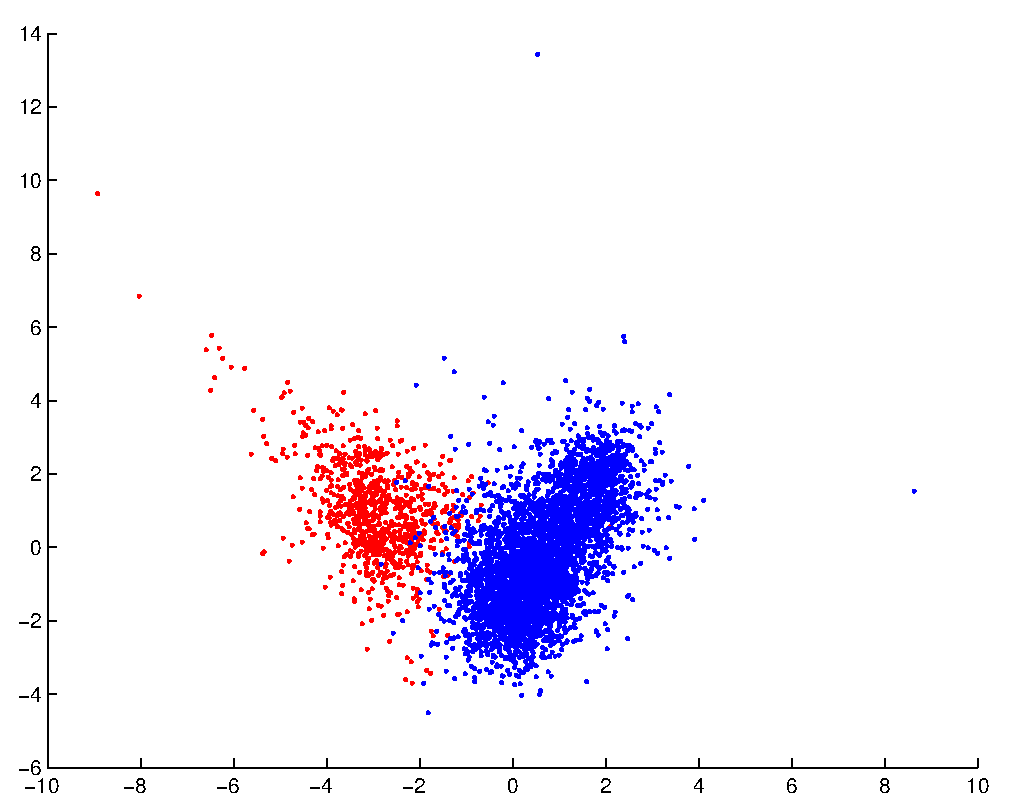
\includegraphics[width=0.5\textwidth]{trainingpca}
\caption{PCA projection of the training dataset}
\label{fig:color_training_pca}
\end{figure}

\begin{figure}[H]
\centering
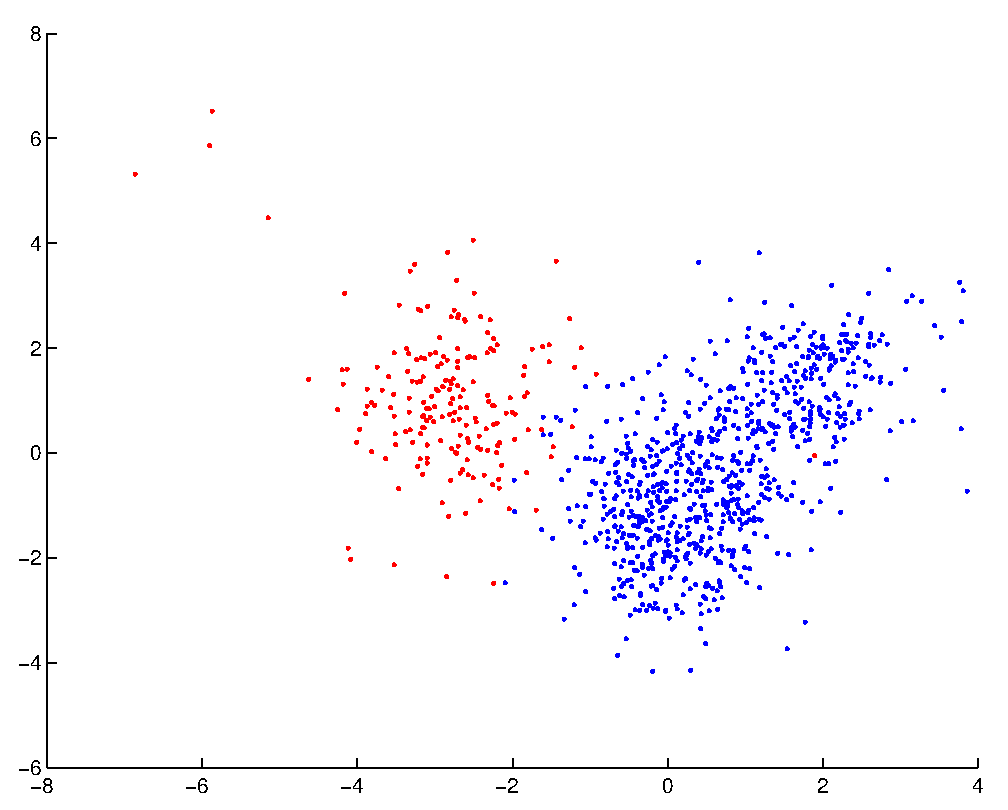
\includegraphics[width=0.5\textwidth]{testpca}
\caption{PCA projection of the testing dataset}
\label{fig:color_testing_pca}
\end{figure}

\subsubsection{kNN cross-validation}

A cross-validation procedure was performed to find and optimal value for the parameter $k$ in the 
kNN -algorithm. Both the error rate and f-score were computed for each $k$. In general the value
of $k$ is odd, so that there will not be votes that result into ties. The results are given in
Fig. \ref{fig:knncrossval}.

\begin{figure}[H]
\centering
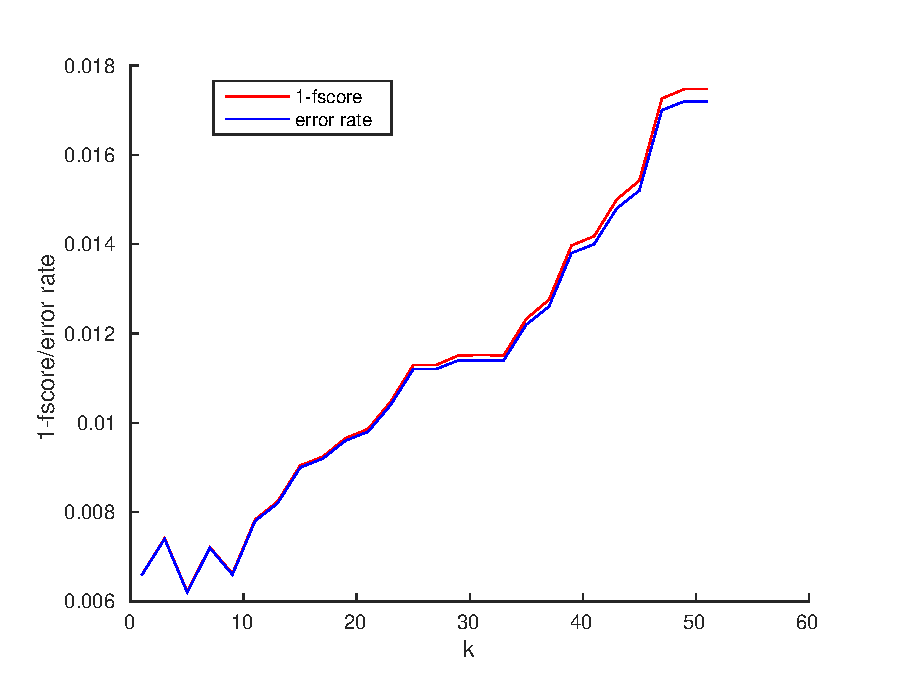
\includegraphics[width=0.5\textwidth]{knncrossval}
\caption{Cross-validation for the parameter of kNN}
\label{fig:knncrossval}
\end{figure}

\subsubsection{Random forest cross-validation}

For random forests, the size of forests and the amount of values in one tree has to be determined.
With a too large forest, computation becomes very slow. Forests of two different sizes were used
for cross-validation over the amount of variables in one tree ($k$). The results with a forest of 400
trees are given in Fig. \ref{fig:RF400crossval} and the results of with a forest of 1000 trees
are given in Fig. \ref{fig:RF1000crossval}.

\begin{figure}[H]
\centering
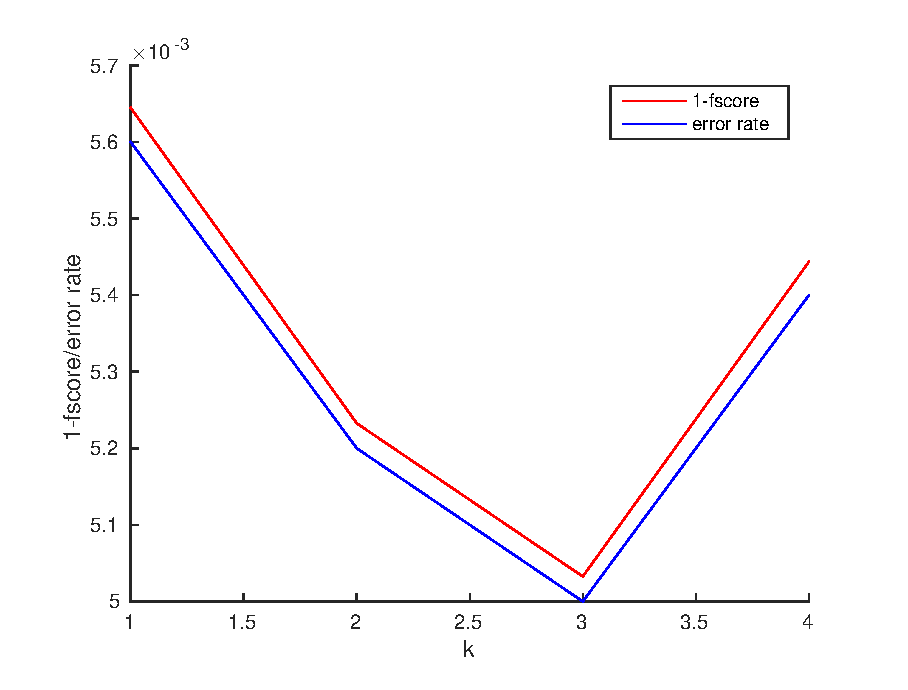
\includegraphics[width=0.5\textwidth]{randforcrossval400}
\caption{Cross-validation for the parameter of the random forest, forest size 400}
\label{fig:RF400crossval}
\end{figure}

\begin{figure}[H]
\centering
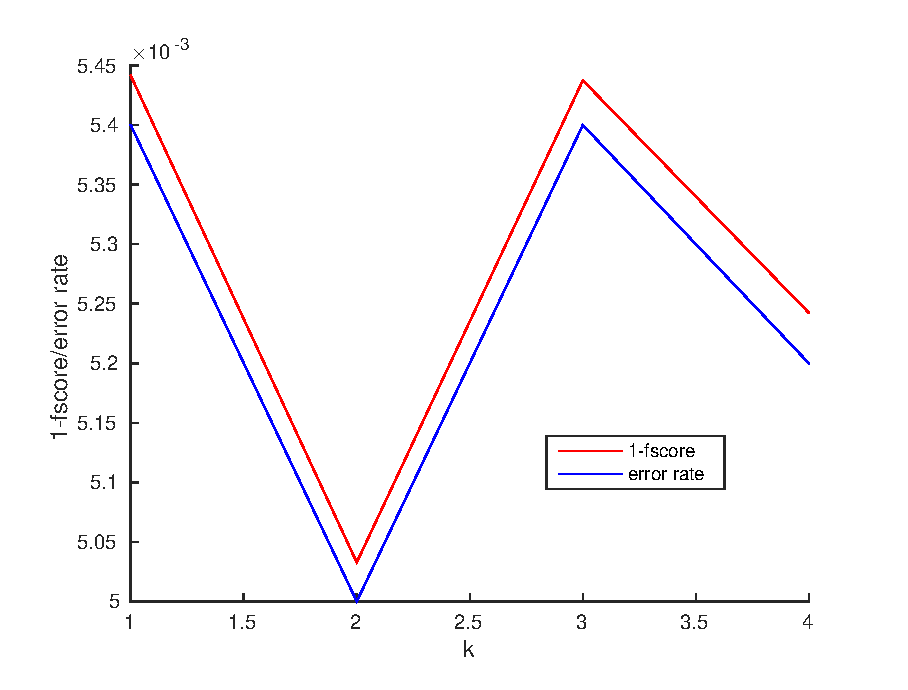
\includegraphics[width=0.5\textwidth]{randforcrossval1000}
\caption{Cross-validation for the parameter of the random forest, forest size 1000}
\label{fig:RF1000crossval}
\end{figure}

\subsubsection{PCA with linear discrimination}

The effects of a PCA algorithm was tested on the given data with cross-validation. 
For this analysis, linear discrimination was used. It was tested with all different
amounts of PCA-components ($k$), to check, whether some of the given data is redundant.
The results are presented in Fig. \ref{fig:lindiscrpca}.

\begin{figure}[H]
\centering
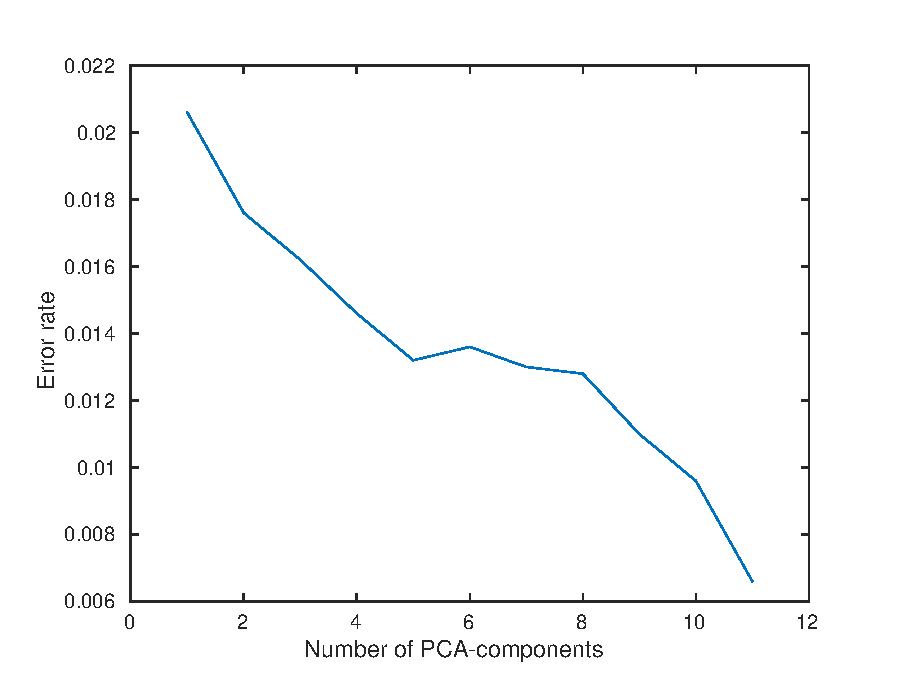
\includegraphics[width=0.5\textwidth]{lindiskrpca}
\caption{Cross-validation for the amount of used PCA components}
\label{fig:lindiscrpca}
\end{figure}

\subsubsection{Cross-validation between algorithms}

To determine, which algorithms should be used for the final evaluation a 10-fold cross-validation was performed. As a result, error values and f-scores were obtained.
These are useful for estimating the actual performance of the algorithms in a test set. The parameter of 
kNN is set to $k = 5$ and for the random forest 400 trees are used with two variables in each tree. These
selections are based on cross-validation and are motivated in the discussion-section.

Table~\ref{table:color_validation} shows the mean error rates and f-scores for each evaluated algorithm obtained in validation. The values are averaged over each
cross-validation partition on the training data.

\begin{table}[H]
\caption{Color prediction - validation}
\label{table:color_validation}
\begin{tabular}{lll}
\textbf{Method} & \textbf{Error rate} & \textbf{F-score}\\
\midrule
Dummy & 18.12\% & 0.7373 \\
\\
\multicolumn{3}{c}{\textbf{Naive Gaussian}} \\
Uniform prior & 27.44\% & 0.7560 \\
Proportional prior & 22.90\% & 0.7820 \\
\\
\multicolumn{3}{c}{\textbf{Multivariate Gaussian}} \\
Uniform prior & 2.22\% & 0.9782 \\
Proportional prior & 1.94\% & 0.9809 \\
\\
\multicolumn{3}{c}{\textbf{Other methods}} \\
Linear discrimination & 0.66\% & 0.9934 \\
$5$ nearest neighbours & 0.62\% & 0.9938 \\
Random forest & 0.50\% & 0.9950 \\
Hybrid & 0.38\% & 0.9962 \\

\end{tabular}
\end{table}

\subsubsection{Testing}

To study the true performance of the final model(s), f-scores and error rates were calculated also using the test set. To view
the goodness of the choice of algorithms by cross-validation, these were calculated for all the methods used. 
Table~\ref{table:color_testing} shows the error rates and f-scores for each algorithm studied.

\begin{table}[H]
\caption{Color prediction - testing}
\label{table:color_testing}
\begin{tabular}{lll}
\textbf{Method} & \textbf{Error rate} & \textbf{F-score}\\
\midrule
Dummy & 19.60\% & 0.717 \\
\\
\multicolumn{3}{c}{\textbf{Naive Gaussian}} \\
Uniform prior & 30.00\% & 0.730 \\
Proportional prior & 25.60\% & 0.756 \\
\\
\multicolumn{3}{c}{\textbf{Multivariate Gaussian}} \\
Uniform prior & 2.30\% & 0.977 \\
Proportional prior & 1.90\% & 0.981 \\
\\
\multicolumn{3}{c}{\textbf{Other methods}} \\
Linear discrimination & 0.30\% & 0.997 \\
$5$ nearest neighbours & 0.40\% & 0.996 \\
Random forest & 0.40\% & 0.996 \\
Hybrid & 0.20\% & 0.998 \\

\end{tabular}
\end{table}

\subsection{Prediction of Quality}

Similarly to the procedures in the type prediction, the available algorithms were studied with both cross-validation and using the test set. 
The performance of the linear discriminant, quadratic discriminant, support vector machine, k nearest neighbors and random forest
classification algorithms, as well as the random forest and linear least squares regression algorithms were tested.
Since the majority of the test observations are of quality 4, a natural dummy model is one that assumes that all wines have the quality of 4.
It is also included in the results.

The training and testing datasets can be visualized by projecting into a two-dimensional plane using principal component analysis. The 
two most important components of the data are presented in figures~\ref{fig:quality_training_pca} (training set) and~\ref{fig:quality_testing_pca}
(test set).
The black dots mark a score of 4, red as score that is larger than 4 and blue a score that is smaller than 4.
For each evaluated algorithm, the classification error rate, the F-score, and the \emph{distance} defined by Eq. \eqref{distmetric}. In addition, the predictions are shown on a PCA projection
of the observations. These projections can be found in appendix \ref{appendix:qualitypcakuvet}.

Typical code used for this task is given in appendix \ref{appendix:qualitycode}. This shows the cross-validation of all algorithms and
contains all the essential information of the analysis.

\begin{figure}[H]
\centering
\includegraphics[width=0.5\textwidth]{qpcatraining}
\caption{PCA projection of the training dataset. Blue indicates bad and red good quality.}
\label{fig:quality_training_pca}
\end{figure}

\begin{figure}[H]
\centering
\includegraphics[width=0.5\textwidth]{qpcatesting}
\caption{PCA projection of the testing dataset. Blue indicates bad and red good quality.}
\label{fig:quality_testing_pca}
\end{figure}

\subsubsection{kNN cross-validation}

A cross-validation procedure was performed to find an optimal value for the parameter $k$ with the 
kNN -algorithm. The procedure was similar to that of the quality prediction. The largest difference is
the quantity that is being predicted. The results are given in
Fig. \ref{fig:knnqcrossval}.

\begin{figure}[H]
\centering
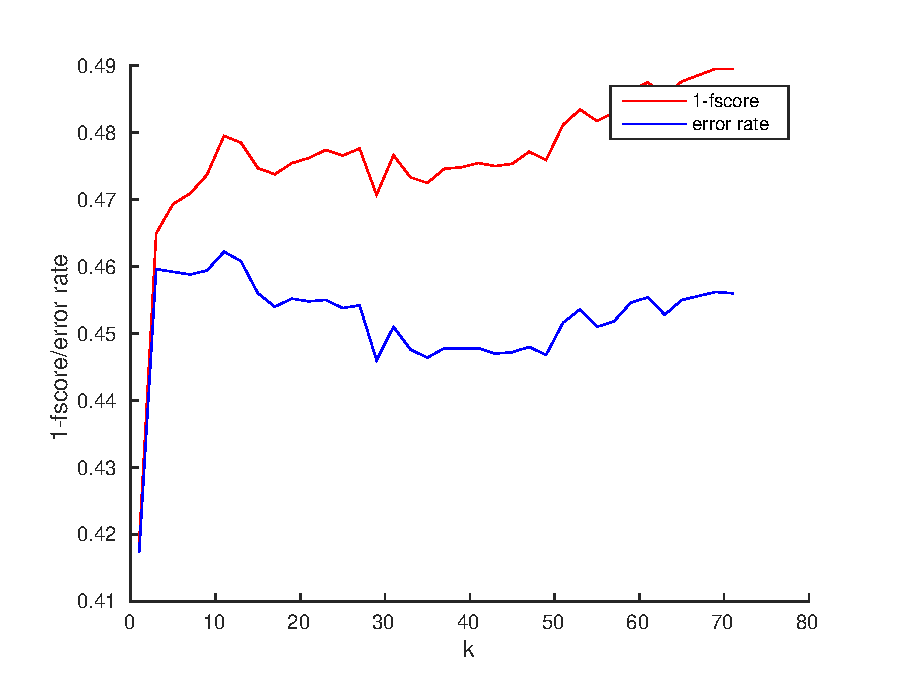
\includegraphics[width=0.5\textwidth]{knnqcrossval}
\caption{Cross-validation for the parameter of kNN}
\label{fig:knnqcrossval}
\end{figure}

\subsubsection{Random forest cross-validation}

For the random forest, the size of forests and the amount of values in one tree has to be again.
Because of the complexity of the problem, a large forest with 1000 trees is used. Cross-validation
is done to test trees that include different amounts of variables ($k$). The results are given in Fig. 
\ref{fig:RFqcrossval}.

\begin{figure}[H]
\centering
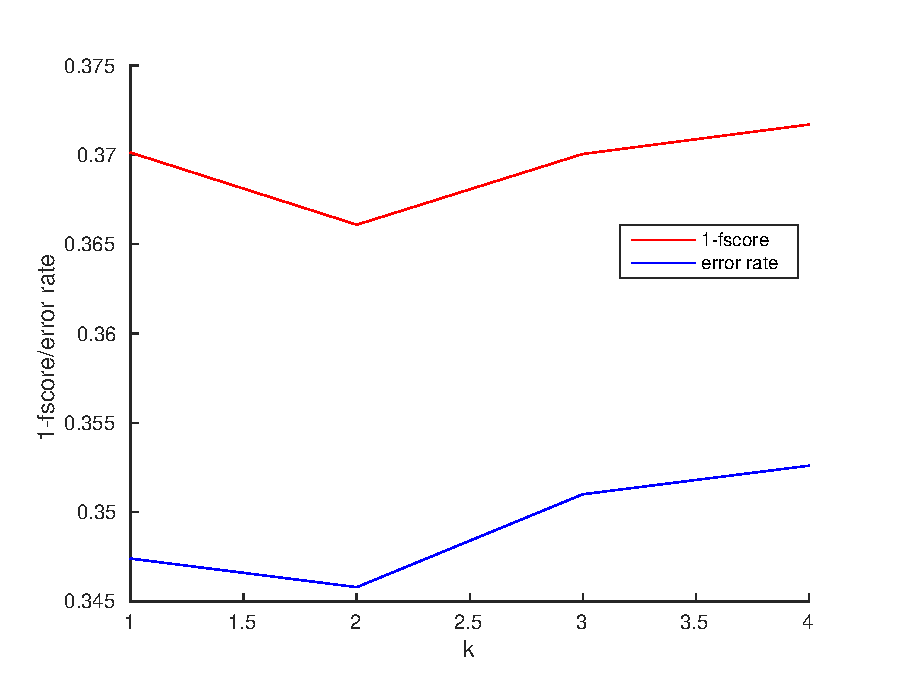
\includegraphics[width=0.5\textwidth]{RFqcrossval}
\caption{Cross-validation for the parameter of the random forest, forest size 400}
\label{fig:RFq1000crossval}
\end{figure}

\subsubsection{Validation}

The cross-validation results are most important while making decisions of the final models. Thus, the results of cross-validation are reported carefully for all algorithms.
Table~\ref{table:quality_validation} shows the mean error rates, f-scores, and \emph{distances} for each evaluated algorithm when run against the validation data. The values are averaged over each
cross-validation partition of the training data.

\begin{table}[H]
\caption{Quality prediction - validation}
\label{table:quality_validation}
\centering
\begin{tabular}{llll}
\multicolumn{3}{l}{\textbf{Method}} \\
\textbf{Error rate} & \textbf{F-score} & \textbf{Distance} \\
\midrule
\multicolumn{3}{l}{Dummy} \\
56.06\% & 0.2685 & 0.0398 \\
\multicolumn{3}{l}{Linear discriminant} \\
46.14\% & 0.5111 & 0.0360 \\
\multicolumn{3}{l}{Quadratic discriminant} \\
51.80\% & 0.4787 & 0.0391 \\
\multicolumn{3}{l}{Support vector machine} \\
46.96\% & 0.4576 & 0.0368 \\
\multicolumn{3}{l}{$1$ nearest neighbor} \\
41.74\% & 0.5810 & 0.0377 \\
\multicolumn{3}{l}{Random forest} \\
35.06\% & 0.6293 & 0.0311 \\
\multicolumn{3}{l}{Random forest (regression)} \\
39.62\% & 0.5742 & 0.0320 \\
\multicolumn{3}{l}{Linear least squares} \\
47.24\% & 0.4907 & 0.0362 \\
\end{tabular}
\end{table}

\subsubsection{Testing}

All the algorithms were at the testing phase. Thus, it is easy to view whether the cross validation has been a good measure of precision or not.
Table~\ref{table:quality_testing} shows the mean error rates, f-scores, and \emph{distances} for each evaluated algorithm when run against the testing data.

\begin{table}[H]
\caption{Quality prediction - testing}
\label{table:quality_testing}
\centering
\begin{tabular}{llll}
\multicolumn{3}{l}{\textbf{Method}} \\
\textbf{Error rate} & \textbf{F-score} & \textbf{Distance} \\
\midrule
\multicolumn{3}{l}{Dummy} \\
59.20\% & 0.2356 & 0.0286 \\
\multicolumn{3}{l}{Linear discriminant} \\
47.70\% & 0.4945 & 0.0249 \\
\multicolumn{3}{l}{Quadratic discriminant} \\
53.70\% & 0.4541 & 0.0279 \\
\multicolumn{3}{l}{Support vector machine} \\
50.10\% & 0.4279 & 0.0264 \\
\multicolumn{3}{l}{$1$ nearest neighbor} \\
41.90\% & 0.5789 & 0.0259 \\
\multicolumn{3}{l}{Random forest} \\
35.60\% & 0.6285 & 0.0216 \\
\multicolumn{3}{l}{Random forest (regression)} \\
39.50\% & 0.5757 & 0.0226 \\
\multicolumn{3}{l}{Linear least squares} \\
48.80\% & 0.4740 & 0.0249 \\
\end{tabular}
\end{table}

%------------------------------------------------

\section{Discussion and Conclusions}
% 4/80 p
%Pohdinnot, results:issa vain raportointi, ei pohdintaa. Lopetus.

The analysis was strongly divided into type and quality prediction.
Even if there were much differences, some of the knowledge gained in the color prediction
was helpful also with the more complex task to augur the quality.

\subsection{Prediction of type}

As can be seen in Fig. \ref{fig:color_training_pca}, the type of the wines is already quite well separated into two 
classes, when the two primary components are studied. However, the division is not complete and some effort is needed
to obtain an optimized prediction model.

The general cross-validation results are given in Table \ref{table:color_validation}. When the error
rate is studied, the dummy model performed better than the univariate Gaussian estimator. However, when the more complex estimator (f-score) is used,
also the one-dimensional Gaussian estimator gives better results than the naive model. In contrast to these simple models,
the multivariate Gaussian estimator performed surprisingly well in terms of both the error rate and the f-score.
However, it should be noted that this is not nearly optimal model for the data in use. The non-Gaussian behavior
of the data can be easily observed and therefore there is a strong inductive bias present. Both in the case of the
multivariate and the single variable Gaussian estimator, using a prior was useful. This is not surprising, because
with weaker models using a prior is likely to have a positive effect.

Three potentially good models were taken into the actual group of possible final models. For two of these some preliminary
parameter choices had to be made. As can be seen in Fig. \ref{fig:knncrossval}, $k = 5$ seems is the optimal choice
for the kNN algorithm and thus it is used in the analysis. The case of the random forest algorithm is more complicated, see
Figs. \ref{fig:RF400crossval} (400 trees) and \ref{fig:RF1000crossval} (1000 trees).
A forest with 1000 trees is already relatively slow to use in a study and therefore no larger forests were used. 

At 400
trees 3 variables in a tree seems to be favorable but at 1000 trees 2 variables in a tree is significantly better and 3 variables
in a tree is unfavorable. Additionally, there seems to be some statistical noise in the results. Thus, with some risk it is
decided to use two variables in a tree, with a forest of 400 trees. This is potentially a worse choice than using 3 parameters,
but the difference should not be large. As a curiosity, it is informative to observe that the error rate and the difference between the
f-score and 1 are close to each other, when the f-score is close to 1.

While experimenting with these methods, it was observed that all of the more involved models performed quite well. Thus it was
decided to combine all the three of them. There might be better ways to combine algorithms and at an error rate this low, it is
hard to have a significant enhancement shown in the final results. A cross-validation was performed to choose coefficients for
the probabilities of these three model (random forest, kNN and linear discrimination). The (cross-validated) error rate for the final hybrid model
is lower than that of any single model as well as the f-score.

A separate PCA-analysis was performed with linear discrimination. As it can be seen from Fig. \ref{fig:lindiscrpca}, there is no
benefit gained by reducing the amount of dimensions. This is useful to acknowledge, since unnecessary variables would
account for excess complexity. Here only the error rate is studied, which is sufficient for this study.

By viewing Fig. \ref{fig:color_testing_pca} that is a PCA-analysis for the test set, it can be seen that the color is quite similarly 
distributed in the test set as in the training set. Additionally, from Table \ref{table:color_testing} it is seen that the f-score and
error rate are even better in the test set than the cross-validated numbers imply. Also, we observe that the cross-validated results and the
test set results are in general close to each other. Thus, the whole procedure of evaluating different models seems to be successful,
at least in the context of the given test dataset. The final error is of the order of a couple of misclassifications. From Appendix
\ref{appendix:colorpcakuvet} it can be seen that at least one red wine is somewhat in the middle of white wines. This could be caused for instance 
by a very untypical wine or a misclassification while recording the data. Thus, it is not reasonable to expect a much better success rate. Random
errors can be always present for different reasons, even if the model was optimal.

\subsection{Prediction of Quality}

As it was originally hypothesized, determining the quality is a much more challenging task than the color prediction. This can be seen from Fig.
\ref{fig:quality_training_pca}, where the black dots mark a ranking 4, blue dots a lower ranking and red dots a higher ranking. There is not a
very clear separation present in this figure between different sections, in contrast to the quality of wines. This augurs a troublesome
process of method optimization.

It was necessary to find fitting parameters for the kNN algorithm and for the random forest algorithm. From Fig. \ref{fig:knnqcrossval}
it can be seen that $k = 1$ would be the preferable parameter value in this case for kNN. This choice is not that good, if the algorithms are to be combined.
With $k = 1$ the probability estimates are not useful. However, at this phase it is not known, if the algorithm is going to be combined with some other
algorithm. Thus, it is sensible to choose initially $k = 1$ and make further considerations later. For the random forest algorithm, 
a forest of 1000 trees was chosen directly, to deal with the complexity. A cross-validation over variable-amounts was done
and the results can be viewed in Fig. \ref{fig:RFq1000crossval}. Here it is obvious, that two variables in a tree gives the optimal results.

This time only the dummy model was hypothetically worse than the others. There was no way to predict differences between the other models. The 
cross-validation errors are shown in Fig. \ref{table:quality_validation}. In terms of the error rate, the dummy model performed quite well, but its 
f-score is very low. Many of the models were badly performing with the present problem. The linear least squares model was bad 
in terms of f-score and error rate and also its mean square error is not exceptionally good. On the other hand, the random forest for regression
had the second best performance. However, it was bested by the actual random forest algorithm in all the goodness measures. Thus, at least with
the present level of analysis regression models were less favorable in all ways, and the problem can be safely done by classification.

Only the linear discriminant of the methods involving dicrimination obtained an f-score greater than 0.5 and even this with a small marginal.
Apparently the quadratic discrimination model was too complex and also the support vector machine was not of use in this case. It turns out 
that only kNN with $k = 1$ can get somewhat close to the performance of the random forest algorithm for classification. Having this in mind,
the kNN is incompatible for algorithm fusion, since $k = 1$ and the performance would be worse with for instance $k = 3$. Thus it seems that
no benefit is gained by fusing algorithms. The random forest model for classification is in this case the final model. The results are not
excellent, but at least the ranking could be predicted to some degree. It seems that a much more involved model is required.

By viewing Fig. \ref{fig:quality_testing_pca} (PCA for the test set), it can be seen that once again the test set resembles the training set.
From the table \ref{table:quality_testing} it is determined that the cross-validation estimates were accurate in the context of the values
obtained by testing. Thus, it was instructive to use only the random forest algorithm as the final model. There is an error rate of approximately
$35 \%$ left in the data, but this is not disastrous with data that are this complex.

\subsection{Final Remarks}

In general the task of type prediction was completed well, including a small error rate. Similar results could have been
achieved with other algorithms, but there is no reason to expect that they would have performed in a much better way. Even this task did not seem 
to be that simple, since eleven variables are fully needed for this analysis. On the contrary, the task of predicting the quality was
complicated. Even powerful algorithms were stuck with high error rates.

The best performing algorithm was the random forest for classification. It is an ensemble method and therefore it is possible that by applying
ensemble techniques to other algorithms, better result could be obtained. Still, it is not reasonable to assume that some algorithm would obtain
as low error rates as in the case of type classification. This could be explained by many factors. For instance, it is possible that there was not 
a sufficient amount of variables supplied. The human taste is complex and the requirement for more data could explain the quality
of the results. On the other hand, it is possible that the quality ranking is not completely deterministic. The rankings are likely to be given by different
groups of wine criticists and the view of ranking varies to some extent. It is also possible that due to the complexity of the human
taste, more involved methods would be necessary to obtain a lower error rate.

The study was successful with the given tasks. A large variety of algorithms was tested out for the sake of diversity.
The wine type was predicted well and also the ranking received somewhat good augurs. The latter could have been better, but in the context of this
analysis the results were sufficient. As a next step, significantly different algorithms could be used. For instance, neural networks could be useful
for an involved analysis. Additionally, some knowledge about wines and the human taste could be useful. By taking into account more facts,
better results could be received. 

All in all, the task of predicting the wine quality functions as a good benchmark for machine learning algorithms. Since
that many common algorithms perform poorly, a good performance implies that a studied algorithm is good at least at some, complex problems.
There remains much to study in the field of machine learning algorithms. Hence it is good to have commonly known hard problems available for testing
new algorithms.

%----------------------------------------------------------------------------------------
%	REFERENCE LIST
%----------------------------------------------------------------------------------------

% 2/80 p
\bibliographystyle{plain}
\bibliography{final_report}{}

%------------------------------------------------
\appendix
% 4/80 p
% koodi-otteita

\section{PCA figures, type prediction}\label{appendix:colorpcakuvet}
PCA projections that show, which predictions have failed for each algorithm.

\begin{figure}[H]
\centering
\includegraphics[width=0.5\textwidth]{colorpca/dummy}
\caption{Color prediction results: dummy}
\end{figure}

\begin{figure}[H]
\centering
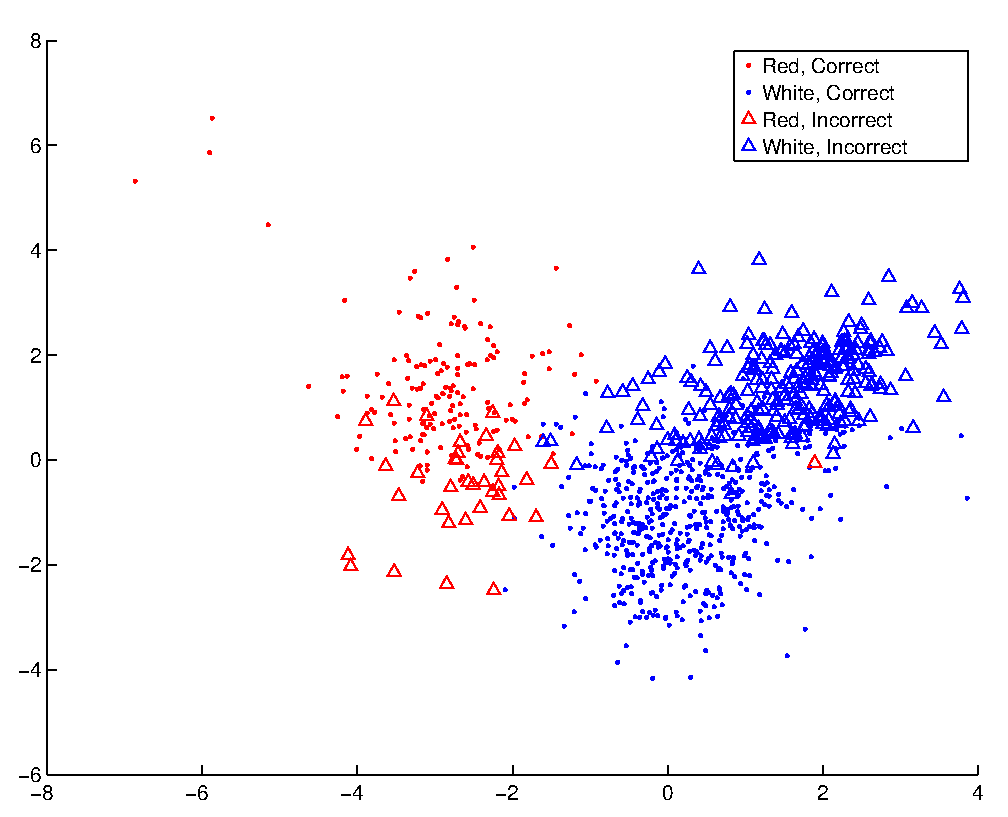
\includegraphics[width=0.5\textwidth]{colorpca/naive_noprior}
\caption{Color prediction results: naive Gaussian, uniform prior}
\end{figure}

\begin{figure}[H]
\centering
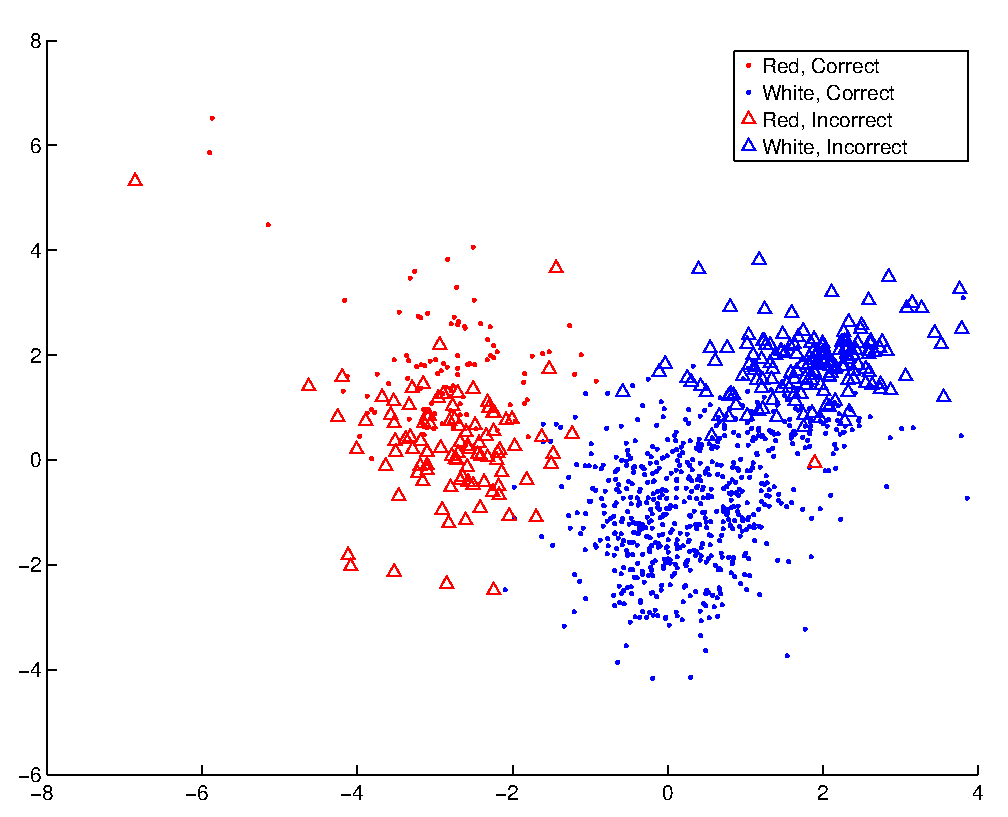
\includegraphics[width=0.5\textwidth]{colorpca/naive_prior}
\caption{Color prediction results: naive Gaussian, proportional prior}
\end{figure}

\begin{figure}[H]
\centering
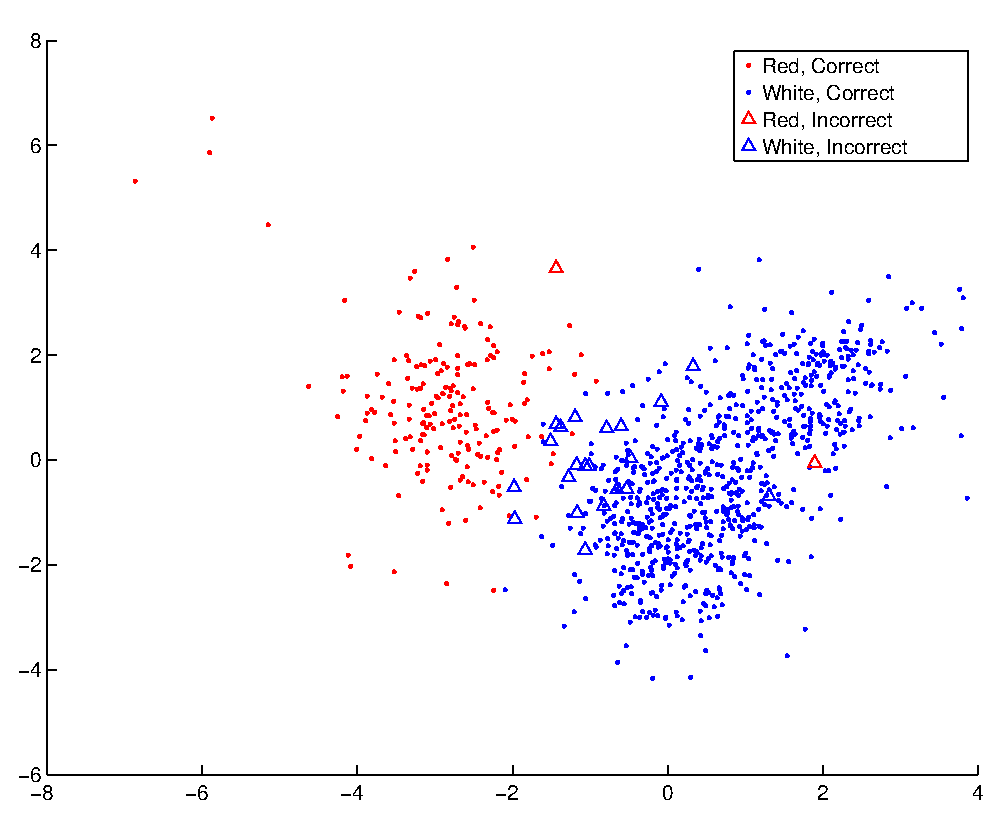
\includegraphics[width=0.5\textwidth]{colorpca/gauss_noprior}
\caption{Color prediction results: multivariate Gaussian, uniform prior}
\end{figure}

\begin{figure}[H]
\centering
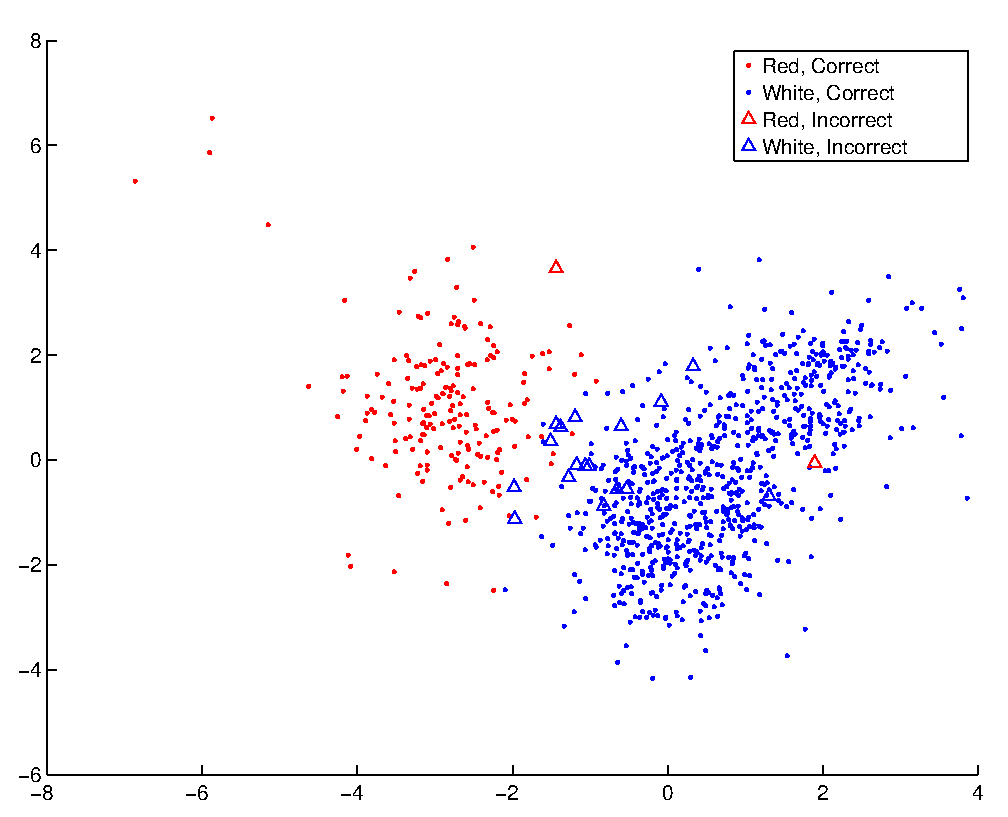
\includegraphics[width=0.5\textwidth]{colorpca/gauss_prior}
\caption{Color prediction results: multivariate Gaussian, proportional prior}
\end{figure}

\begin{figure}[H]
\centering
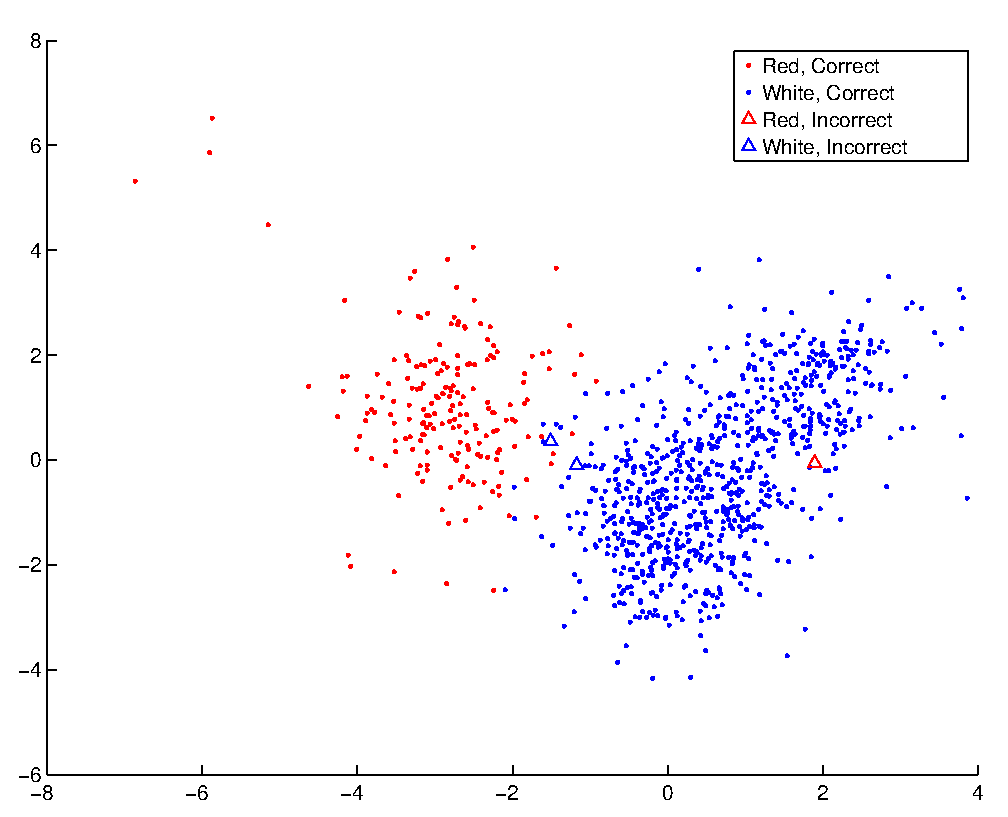
\includegraphics[width=0.5\textwidth]{colorpca/linear_discr}
\caption{Color prediction results: linear discriminant}
\end{figure}

\begin{figure}[H]
\centering
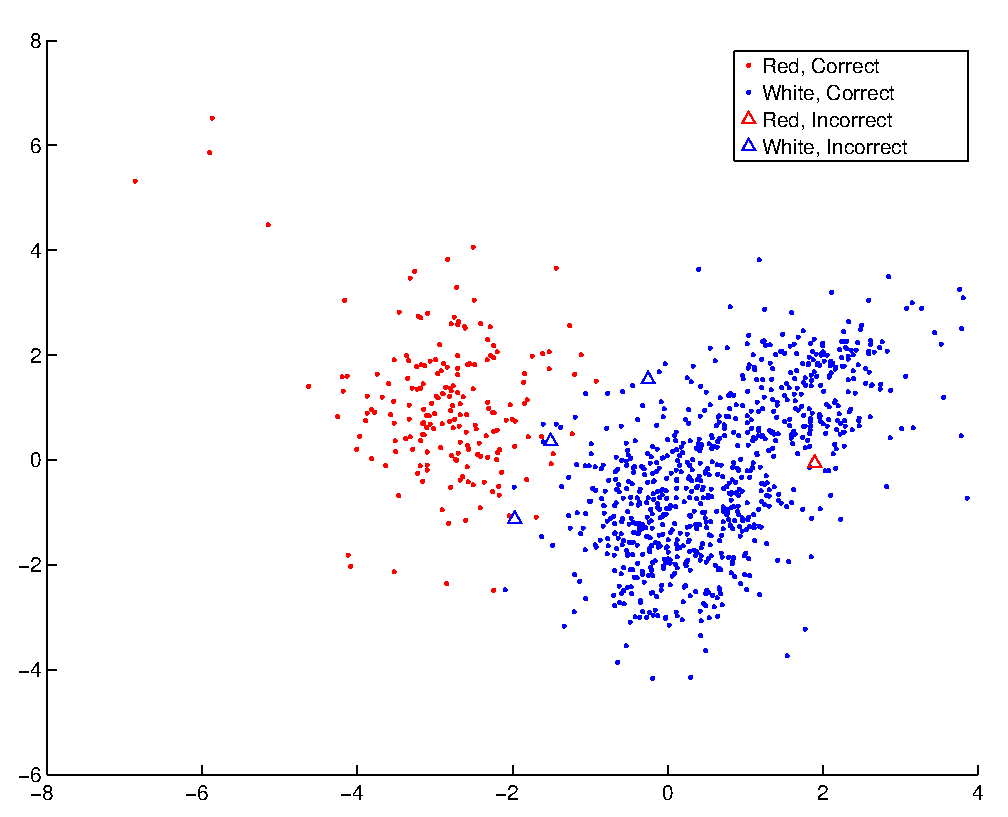
\includegraphics[width=0.5\textwidth]{colorpca/knn5}
\caption{Color prediction results: $5$ nearest neighbors}
\end{figure}

\begin{figure}[H]
\centering
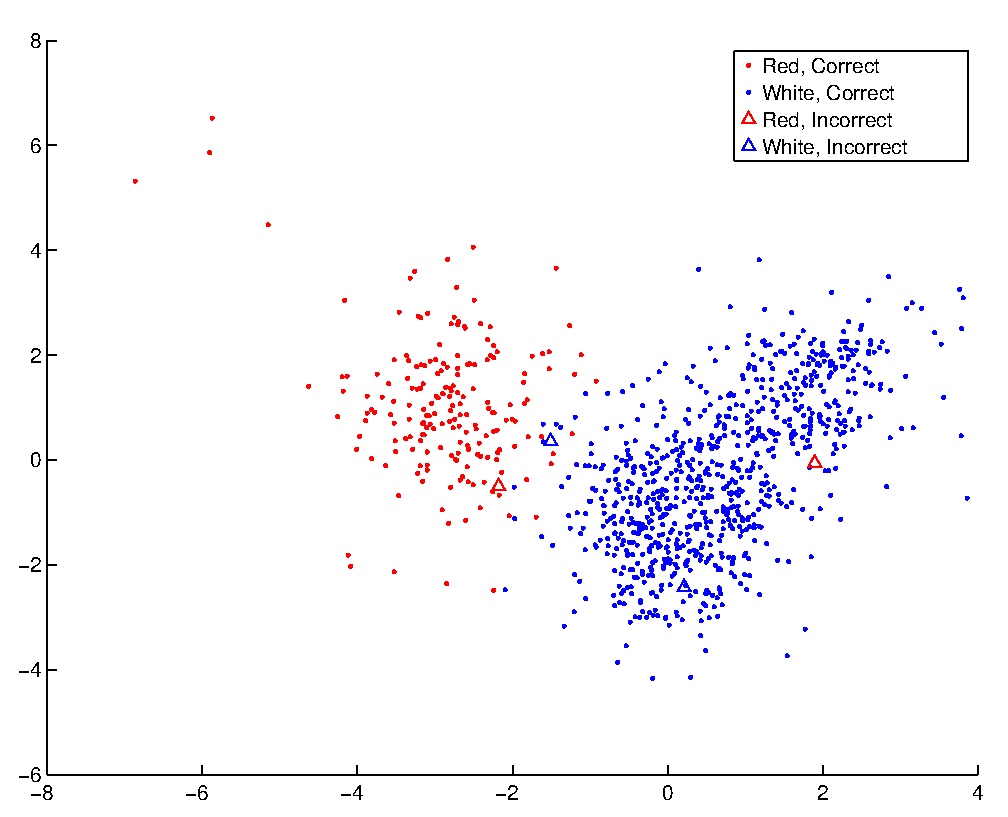
\includegraphics[width=0.5\textwidth]{colorpca/random_forest}
\caption{Color prediction results: random forest}
\end{figure}

\begin{figure}[H]
\centering
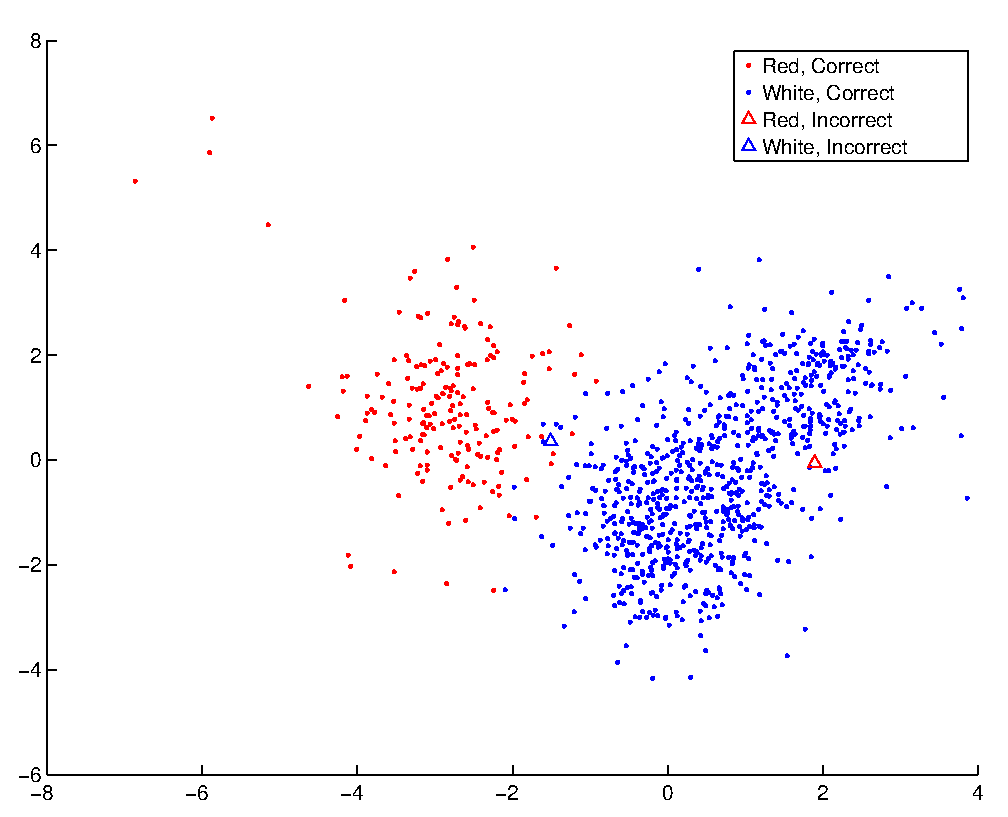
\includegraphics[width=0.5\textwidth]{colorpca/cvv2f_f}
\caption{Color prediction results: hybrid}
\end{figure}

%----------------------------------------------------------------------------------------
\section{PCA figures, quality prediction}\label{appendix:qualitypcakuvet}
PCA projections that show, which predictions have failed for each algorithm.
Dots denote correct predictions, while triangles denote incorrect predictions.
A red triangle means that the predicted quality was too high, while a blue
triangle means that it was too low.

\begin{figure}[H]
\centering
\includegraphics[width=0.5\textwidth]{rankpca/dummy}
\caption{Quality prediction results: dummy}
\end{figure}

\begin{figure}[H]
\centering
\includegraphics[width=0.5\textwidth]{rankpca/lindiscr}
\caption{Quality prediction results: linear discriminant}
\end{figure}

\begin{figure}[H]
\centering
\includegraphics[width=0.5\textwidth]{rankpca/quaddiscr}
\caption{Quality prediction results: quadratic discriminant}
\end{figure}

\begin{figure}[H]
\centering
\includegraphics[width=0.5\textwidth]{rankpca/svm}
\caption{Quality prediction results: support vector machine}
\end{figure}

\begin{figure}[H]
\centering
\includegraphics[width=0.5\textwidth]{rankpca/knn1}
\caption{Quality prediction results: $1$ nearest neighbor}
\end{figure}

\begin{figure}[H]
\centering
\includegraphics[width=0.5\textwidth]{rankpca/randomforest}
\caption{Quality prediction results: random forest}
\end{figure}

\begin{figure}[H]
\centering
\includegraphics[width=0.5\textwidth]{rankpca/randomforestreg}
\caption{Quality prediction results: random forest (regression)}
\end{figure}

\begin{figure}[H]
\centering
\includegraphics[width=0.5\textwidth]{rankpca/ols}
\caption{Quality prediction results: linear least squares}
\end{figure}

\section{Code sample, color prediction}\label{appendix:colorcode}

The following matlab code shows a cross-validation procedure
that tests all the methods used. The code used with the test
set is similar, but it lacks the for-loop that is meant for 
cross-validation.

{\footnotesize

\begin{verbatim}
winefacts = readtable('../training_dataset.csv');
winetests = readtable('../test_dataset.csv');

tra=4500; val=500; tes=1000;

%% 10-fold cross-validation %%

nerrs = 1:10; npriorerrs = 1:10; gerrs = 1:10; 
gpriorerrs = 1:10;
derrs = 1:10; kerrs = 1:10; terrs = 1:10;

err_rates = repmat([0], 10, 8); 
f_scores = repmat([0], 10, 8); 

for h=1:10
    %% Boundaries for cross-validation
    lower = 1+500*(h-1); upper = 500*h;
    indices = [ 1:(lower-1), (upper+1):5000, ...
      lower:upper ];

    %% Set convenient training and validation sets
    training = winefacts(indices(1:tra),:);
    validation = ...
      winefacts(indices(tra+1:tra+val),:);

    traing = [table2array(training(:,1:11)), ... 
      strcmp(training.type, 'Red')];
    valid = [table2array(validation(:,1:11)), ... 
      strcmp(validation.type, 'Red')];

    %% Prior values, if needed
    rPrior = sum(traing(:,12))/tra; wPrior = ...
      1-rPrior;

    %% Naive (only 1 variable) Gaussian 
    %  discrimination
    m1 = mean(traing(traing(:,12)==1,8)); % Reds
    v1 = var(traing(traing(:,12)==1,8));
    m2 = mean(traing(traing(:,12)==0,8)); % Whites
    v2 = var(traing(traing(:,12)==0,8));

    % With no prior and with prior
    nclass1 = (logDiscrNaive( ...
      valid(:,8),m1,m2,v1,v2,1,1)>0);
    nclass2 = (logDiscrNaive( ...
      valid(:,8),m1,m2,v1,v2,rPrior,wPrior)>0);

    %% Gaussian discrimination
    % Reds
    m1 = mean(traing(traing(:,12)==1,1:11)); 
    v1 = cov(traing(traing(:,12)==1,1:11));
    % Whites
    m2 = mean(traing(traing(:,12)==0,1:11)); 
    v2 = cov(traing(traing(:,12)==0,1:11));

    % No prior and prior
    gclass1=(1:val)'; gclass2=(1:val)'; 
    for i = 1:val
        gclass1(i) = (logDiscrGauss(valid(i,...
	  1:11),m1,m2,v1,v2,1,1)>0);
        gclass2(i) = (logDiscrGauss(valid(i,...
	  1:11),m1,m2,v1,v2,rPrior,wPrior)>0);
    end 
    %% Linear discriminant
    diskr = fitcdiscr(traing(:,1:11),...
      traing(:,12),'DiscrimType','Linear');
    dclass=predict(diskr,valid(:,1:11));

    %% kNN, k=1 or k=3
    kNN = fitcknn(traing(:,1:11),traing(:,12), ...
      'Distance','mahalanobis','NumNeighbors',3);
    kclass=predict(kNN,valid(:,1:11));

    %% Random forest 30
    BaggedTreeEns = TreeBagger(200,traing(:,...
      1:11),traing(:,12),'NVarToSample',2);
    [tclass,treeProbs]=predict(BaggedTreeEns,...
      valid(:,1:11));
    tclass = round(treeProbs(:,2));
    
    %% DUMMY

    dummyclass = repmat([0], size(valid, 1), 1);

    %% Standard errors
    nerrs(h) = sum( nclass1 ~= valid(:,12) )/val;
    npriorerrs(h) = sum( nclass2 ~= valid(:,12) )/val;
    gerrs(h) = sum( gclass1 ~= valid(:,12) )/val;
    gpriorerrs(h) = sum( gclass2 ~= valid(:,12) )/val;
    derrs(h) = sum( dclass ~= valid(:,12) )/val;
    kerrs(h) = sum( kclass ~= valid(:,12) )/val;
    terrs(h) = sum( tclass ~= valid(:,12) )/val;

    fprintf('-- h = %d --\n', h);

    [err_rates(h, 1), f_scores(h, 1)] = ... 
      errplotg(valid, nclass1, 'naive_noprior');
    [err_rates(h, 2), f_scores(h, 2)] = ...
      errplotg(valid, nclass2, 'naive_prior');
    [err_rates(h, 3), f_scores(h, 3)] = ...
      errplotg(valid, gclass1, 'gauss_noprior');
    [err_rates(h, 4), f_scores(h, 4)] = ...
      errplotg(valid, gclass2, 'gauss_prior');
    [err_rates(h, 5), f_scores(h, 5)] = ...
      errplotg(valid, dclass, 'linear_discr');
    [err_rates(h, 6), f_scores(h, 6)] = ...
      errplotg(valid, kclass, 'knn3');
    [err_rates(h, 7), f_scores(h, 7)] = ...
      errplotg(valid, cellfun(@str2num,tclass), ...
      'random_forest');
    [err_rates(h, 8), f_scores(h, 8)] = ...
      errplotg(valid, dummyclass, 'dummy');
end

\end{verbatim}

}

\section{Code sample, quality prediction}\label{appendix:qualitycode}

The following matlab code shows a cross-validation procedure
that tests all the methods used. The code used with the test
set is similar, but it lacks the for-loop that is meant for 
cross-validation.

{\footnotesize

\begin{verbatim}

winefacts = readtable('../training_dataset.csv');
winetests = readtable('../test_dataset.csv');

tra=4500; val=500; tes=1000;

%% 10-fold cross-validation %%

derrs = zeros(10,3); qderrs = zeros(10,3); 
serrs = zeros(10,3); trerrs = zeros(10,3); 
kerrs = zeros(10,3); lerrs = zeros(10,3); 
terrs = zeros(10,3); nerrs = zeros(10,3);

for h=1:10
    %% Boundaries for cross-validation
    lower = 1+500*(h-1); upper = 500*h;
    indices = [ 1:(lower-1), ... 
      (upper+1):5000, lower:upper ];

    %% Set convenient training and validation sets
    training = winefacts(indices(1:tra),:);
    validation = winefacts(...
      indices(tra+1:tra+val),:);

    traing = [table2array(training(:,1:11)), ... 
      strcmp(training.type, 'Red'), ...
      training.quality];
    valid = [table2array(validation(:,1:11)), ...
      strcmp(validation.type, 'Red'), ...
      validation.quality];

    %% Ultimately naive prediction
    nclass = ones(val,1)*4;
    
    %% Linear discriminant
    diskr = fitcdiscr(traing(:,1:11),...
      traing(:,13),'DiscrimType','Linear');
    dclass=predict(diskr,valid(:,1:11));

    %% Quadratic discriminant
    qdiskr = fitcdiscr(traing(:,1:11),...
      traing(:,13),'DiscrimType','pseudoQuadratic');
    qdclass = predict(qdiskr,valid(:,1:11));
    
    %% SVM
    svm = fitcecoc(traing(:,1:11),traing(:,13));
    sclass = predict(svm,valid(:,1:11));
    
    %% kNN, k=3
    kNN = fitcknn(traing(:,1:11),traing(:,13), ...
      'Distance','mahalanobis','NumNeighbors',3);
    kclass=predict(kNN,valid(:,1:11));

    %% Random forest
    BaggedTreeEns = TreeBagger(1000, ...
      traing(:,1:11),traing(:,13),'NVarToSample',2);
    tclass=predict(BaggedTreeEns,valid(:,1:11));
    tclass=cell2mat(tclass); tclass=tclass-48;

    %% Random forest, regression
    BaggedTreeEns = TreeBagger(1000, ...
      traing(:,1:11),traing(:,13), ...
      'NVarToSample',2,'Method','regression');    
    trclass=round(predict(BaggedTreeEns,...
      valid(:,1:11)));
        
    %% Least squares, regression
    w = lscov(traing(:, 1:11), traing(:, 13));
    lclass = round(valid(:, 1:11) * w);

    %% Standard errors
    nerrs(h,1) = sum( nclass ~= valid(:,13) )/val;
    derrs(h,1) = sum( dclass ~= valid(:,13) )/val;
    qderrs(h,1) = sum( qdclass ~= valid(:,13) )/val;
    serrs(h,1) = sum( sclass ~= valid(:,13) )/val;
    kerrs(h,1) = sum( kclass ~= valid(:,13) )/val;
    terrs(h,1) = sum( tclass ~= valid(:,13) )/val;
    trerrs(h,1) = sum( trclass ~= valid(:,13) )/val;
    lerrs(h,1) = sum( lclass ~= valid(:,13) )/val

    nerrs(h,2) = tot_fscore(nclass,valid(:,13));
    derrs(h,2) = tot_fscore(dclass,valid(:,13));
    qderrs(h,2) = tot_fscore(qdclass,valid(:,13));
    serrs(h,2) = tot_fscore(sclass,valid(:,13));
    kerrs(h,2) = tot_fscore(kclass,valid(:,13));
    terrs(h,2) = tot_fscore(tclass,valid(:,13));
    trerrs(h,2) = tot_fscore(trclass,valid(:,13));
    lerrs(h,2) = tot_fscore(lclass,valid(:,13));

    nerrs(h,3) = meansqerr(nclass,valid(:,13));
    derrs(h,3) = meansqerr(dclass,valid(:,13));
    qderrs(h,3) = meansqerr(qdclass,valid(:,13));
    serrs(h,3) = meansqerr(sclass,valid(:,13));
    kerrs(h,3) = meansqerr(kclass,valid(:,13));
    terrs(h,3) = meansqerr(tclass,valid(:,13));
    trerrs(h,3) = meansqerr(trclass,valid(:,13));
    lerrs(h,3) = meansqerr(lclass,valid(:,13));
end

\end{verbatim}

}

\end{multicols}

\end{document}
